\chapter{Introduction}
\label{ch:introduction}
\setcounter{footnote}{0}
The Greek philosopher Heraclitus once said that one constant since the beginning of time is change. However, the fear of change is also a constant. His central claim is summed up in the phrase Panta Rhei ("life is flux"), recognising life's essential, underlying essence as change \parencite{Seibt2022}. Nothing in life is permanent, nor can it be, because the very nature of existence is change. Since times \gls{immemorial}, humans have liked routine, making us feel in control of our lives. When the feeling of loosing control becomes irrational, the ability to control it can become a phobia \parencite{PsychTimes}. Someone with a phobia for change feels like they have no control over their lives due to constant change. These people tend to live in the past and are unwilling to progress, often leading to depression, seriously impacting their professional and personal lives. If a society or country rejects change, there could be no growth and progress \parencite{Mark2010}. The inability to change, progress, or grow can result in stagnation.

The Dutch \gls{ps} deals with many changes in its environment. Changes follow one another at lightning speed. These are changes such as new technologies, social developments and political priorities \parencite[p.~1]{Nijssen2018}. In the past, these were internal changes such as improving the financial and human resource processes, implementing a new way to organise and control, and the professionalisation of management processes. In recent years, the external environment placed new and increasingly compelling demands on the functioning of public organisations \parencite[p.~13]{Eck2009}. The \gls{ps} finds it challenging to adapt to the expected speed of change \parencites{Linders2013}[p.~2]{Wiebes2014}[pp.~5--6]{Auditdienst2019a}[p.~8]{Meijer2019}[pp.~1--2]{Tangi2020}. E.g. ''The processes, while solid, cannot withstand the current pace of change; the dependence on emergency solutions and manual work is increasing'' \parencite[p.~2]{Wiebes2014}. Trying to follow the expected speed of change often gets stuck on embedded norms, bureaucracy, processes, and structures \parencite[p.~1]{Tangi2020}. 

''There is a need to invest for an even a better government that can respond adequately and flexibly to unforeseen circumstances.'' was plead to Schippers\footnote{\url{https://en.wikipedia.org/wiki/Edith_Schippers}}\footnote{Schippers was at that time the appointed '\textit{informateur}' (Dutch). An '\textit{informateur}' is responsible to explore possible governing alliances after elections.} \parencite{Secretarissen-generaal2018}. A responsive and adaptive government is needed to deal with this \parencite[pp.~79--81]{Steen2018}. We need to create public organisations that can cope with or even seize opportunities in a dynamic difficult, unpredictable environment \parencite[pp.~1--2]{Nijssen2018}. 

\section{Introduction to antifragile}
\label{sec:introantifragility}
There are different principles to deal with uncertainty and disruptive changes \parencite[pp.~79--81]{Steen2018}. \Citeauthor{Steen2018} uses \textcite{Taleb2012} to discuss several manifestations for dealing with disruptive change. The five manifestations of \textcite{Taleb2012} provide a framework for the conversation about adaptive organisations \parencite[pp.~79--81]{Steen2018}. We have \gls{fragility}, \gls{robustness}, \gls{resiliency}, \gls{agility}, and \gls{antifragility}. Organisations that find it difficult or impossible to deal with changes are fragile. That does not mean that these organisations are not successful. They are often very sturdy, solid and successful. However, a fragile organisation will run into problems if the environment requires something from those organisations beyond the limits of the organisations capabilities. A \gls{robust} organisation absorbs and resists stess, while \gls{resilient} orgranisations move along with stress but bounce back to the status quo. \Gls{agile} organisations avoid stress just in time but do not gain, and with \gls{antifragility} an organisation gets better from stress. Agile is not acknowledged by \textcite{Taleb2012} and is in this context only used by \textcite{Steen2018}. \Gls{resiliency} is mentioned but \textcite{Taleb2012} only uses \gls{fragile}, \gls{robust}, and \gls{antifragile} for his \gls{triad} (\cref{fig:antifragilesimple}).
\begin{figure}[H]
	\centering
	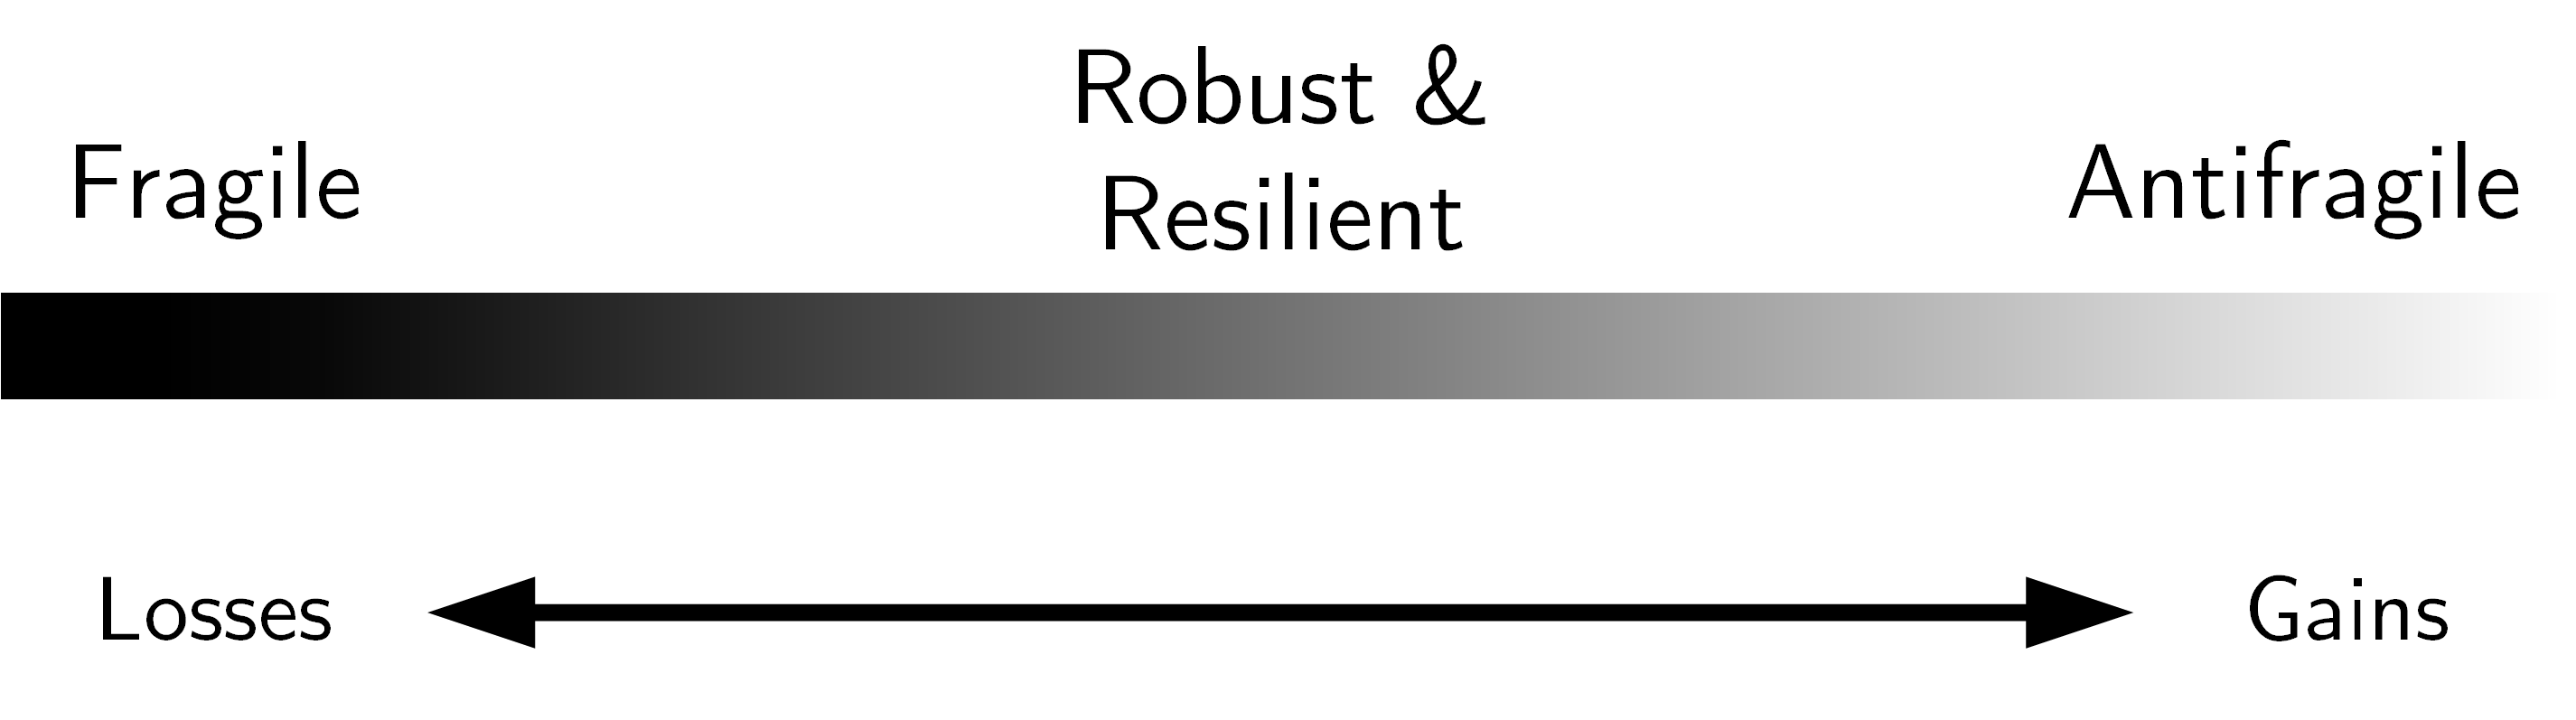
\includegraphics[width=0.6\linewidth]{images/antifragilesimple}
	\caption[The antifragile triad]{The antifragile triad}
	\label{fig:antifragilesimple}
\end{figure}
\textcite{Taleb2012} coined \gls{antifragile} as an answer to what he calls a \gls{blackswan}. \Glspl{blackswan} are large-scale unpredictable, and rare events of massive consequences \parencite[p.~6]{Taleb2012}. For extremely rare events the standard tools of probability and prediction, such as the normal distribution, do not apply since they depend on a large population and past sample sizes that are never available for rare events. \Gls{antifragile} means that a system gains more than it loses.

\section{Introduction to Enterprise Architecture}
\label{sec:introea}
Due to the political environment and social environmental factors, the public sector deals continuously with changes and adjustments to objectives and missions \parencite{EARbaten}. This continuous change confronts policymakers with high demands on their steering skills. Instruments such as the '\acrfull{nora}', '\acrfull{ear}', and '\acrfull{gemma}' make it easier for policymakers to deal with this. \acrshort{nora}, \acrshort{ear}, and \acrshort{gemma} are reference architectures. A reference architecture describes general structures \parencite[p.~8]{Greefhorst2008}. It is not specific to one organisation. Many organisations can use a reference architecture because it is abstract. Abstract architectures are the basis for more specific architectures \parencite[p.~11]{Greefhorst2008}. They are an essential tool for reuse at an architectural level. Therefore, organisations should draw as much as possible from these architectures. We deduct that there are multiple levels of architecture. Some kind of architecture hierarchy. Traditionally, reference architectures and \acrlong{ea} in the \gls{ps} correspond to the \acrshort{nora} terms of content \parencite{NORAfamilie}. The \acrshort{nora} itself is a daughter of the \acrfull{eira} (\cref{fig:architectureviewonion}).
\begin{figure}[H]
	\centering
	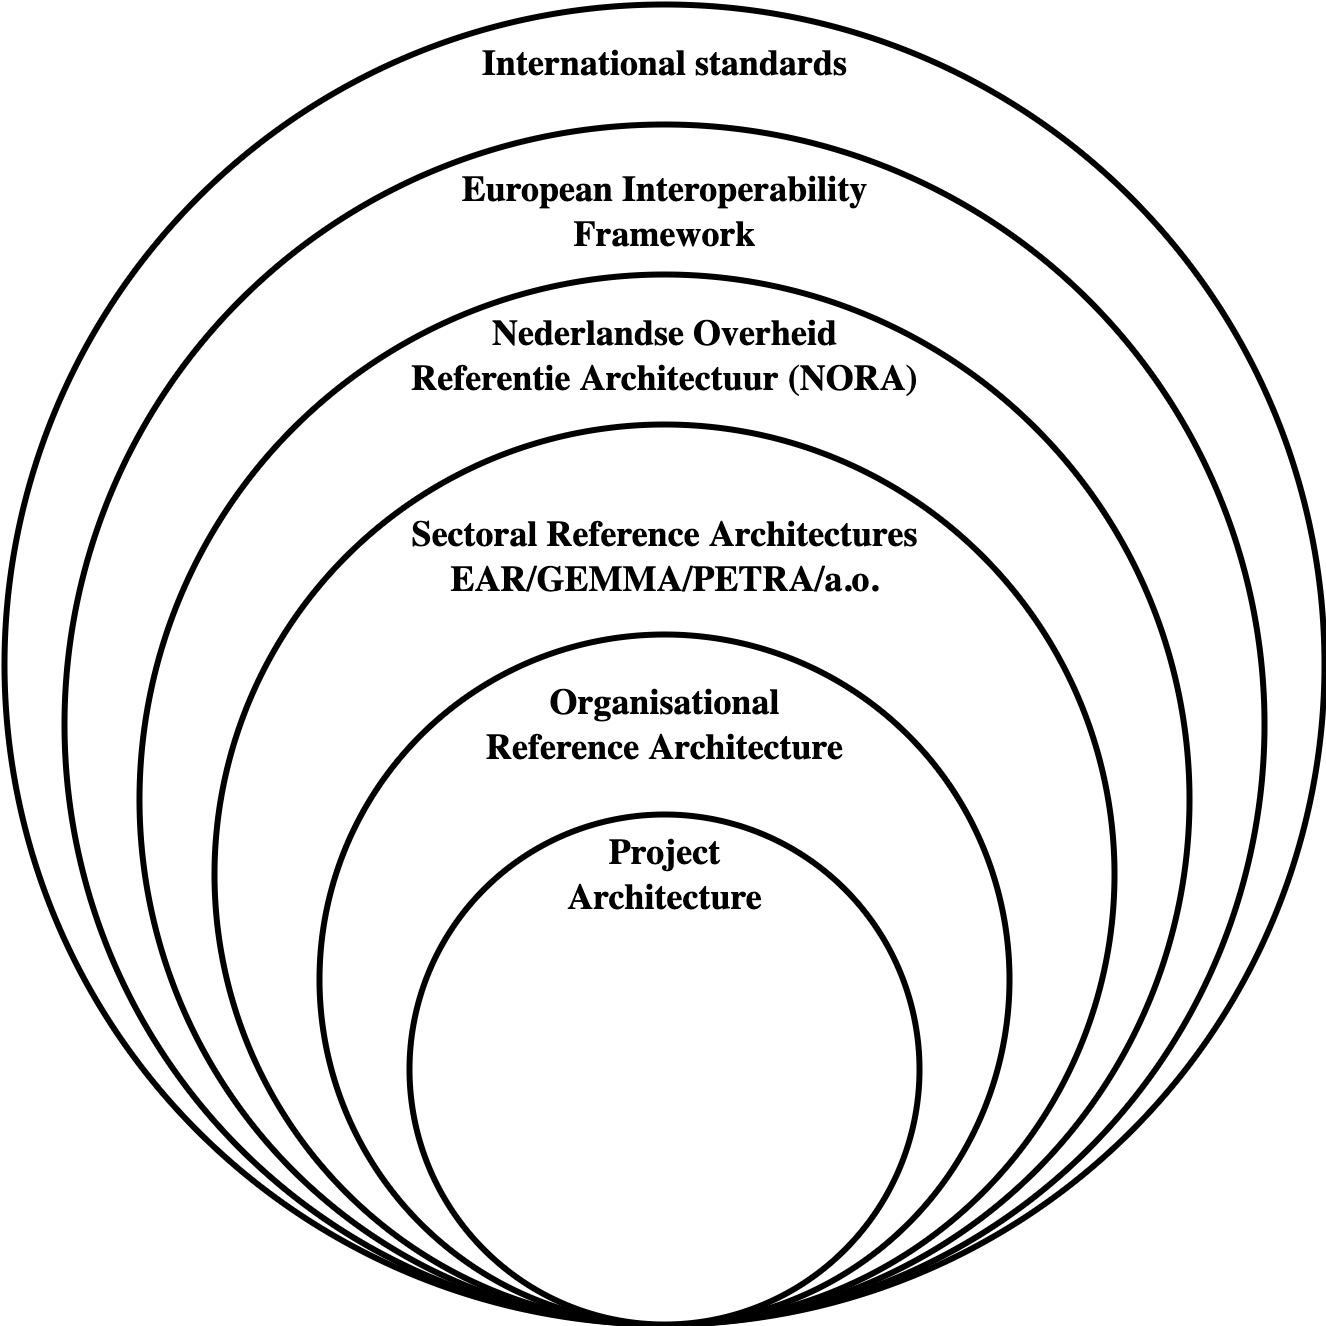
\includegraphics[width=0.5\linewidth]{images/architectureviewonion}
	\caption[Architecture subsidiaries, based on \parencite{Greefhorst2008}]{Architecture subsidiaries, based on \parencite{Greefhorst2008}}
	\label{fig:architectureviewonion}
\end{figure}
The \gls{ps} is used to working with \acrlong{ea} in which \acrlong{ea} the field is between business administration, information science, and computer science which aims to ensure that an organisation develops in the desired direction \parencite{EAwiki}. The \gls{ps} uses \acrlong{ea} to improve interoperability and efficiently use both intra- and inter-organisational systems \parencite[p.~9]{Giskes2020}.

\section{Research}
\label{sec:research}
The \gls{ps} uses \acrlong{ea} to guide and support the \gls{ps} in dealing with continuous change (\cref{sec:introea}). The public sector wants to change to be more adaptive and responsive (\cref{ch:introduction}). To be more adaptive and responsive, \textcite{Steen2018} proposed to use \gls{antifragile} from \textcite{Taleb2012} (\cref{sec:introantifragility}). However, how can we achieve \gls{antifragility} in the \gls{ps} with \acrlong{ea}? What are the possible success factors of \acrlong{ea} and \gls{antifragile} to change the Dutch \gls{ps} to be more adaptive and responsive by using \acrlong{ea} with \gls{antifragility} in the \gls{ps}? One would expect that it is known how \acrlong{ea} can contribute to changing an organisation into a more \gls{antifragile} organisation. However, we could not find information on the combination of \gls{antifragile} and \acrlong{ea} with or without the \gls{ps}. Most research results deal with \gls{antifragility} in application and information architectures. A small number of sources have investigated \gls{antifragility} in combination with organisations and systems. 

We need more information to determine how the \gls{ps} can become more \gls{antifragile} with \acrlong{ea}. We have to determine the success factors that positively influence becoming \gls{antifragile} with \acrlong{ea} (\cref{fig:conceptualmodel}).
\begin{figure}[H]
	\centering
	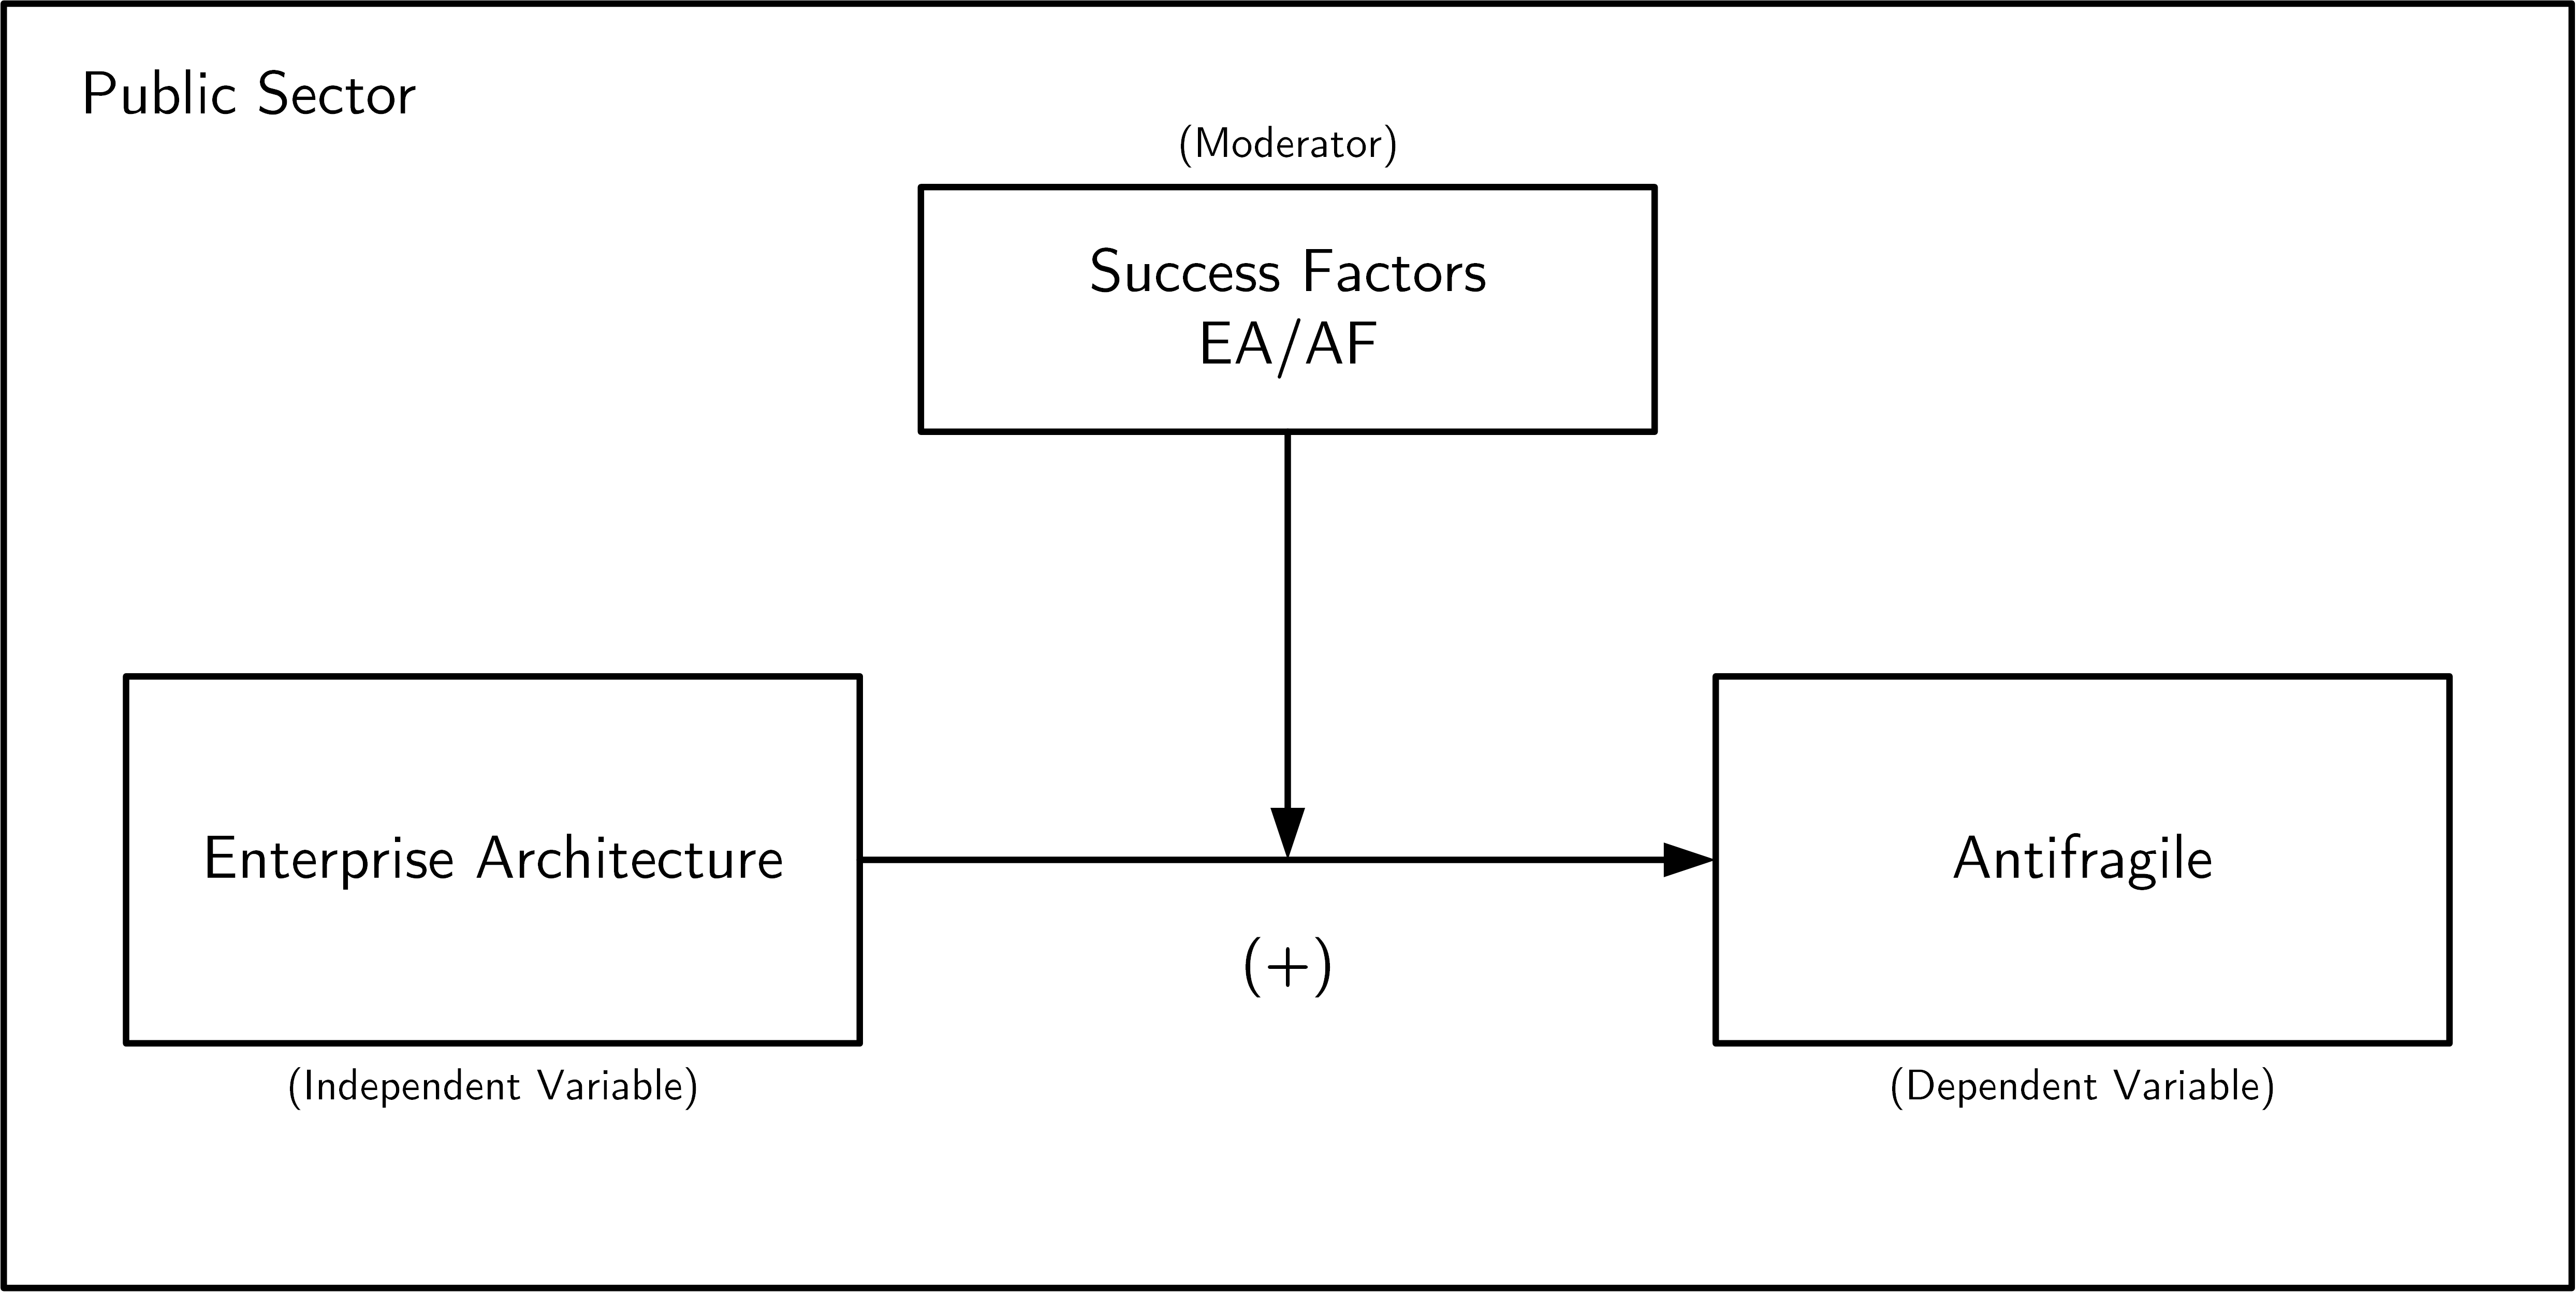
\includegraphics[width=0.7\linewidth]{images/conceptualmodel}
	\caption[Conceptual Research Model]{Conceptual Research Model}
	\label{fig:conceptualmodel}
\end{figure}

\subsection{Research question}
\label{sub:introresearchquestion}
The conceptual research model (\cref{fig:conceptualmodel}) describes the hypothesises that, in the context of the Dutch public sector, there are success factors of \acrshort{ea} and \gls{antifragile} that have a positive influence on the contribution of \acrlong{ea} in achieving \gls{antifragility}. Following the conceptual model, we have the following research question:

\vspace{\baselineskip}
\noindent \emph{''What are success factors that positively influence the contribution of \acrlong{ea} in achieving \gls{antifragility} in the \gls{ps}?''}
\vspace{\baselineskip}

\noindent The following sub-questions support answering the research question:
\begin{enumerate}
	\item{What is the literature saying about the \gls{ps}?}
	\item{What is the literature saying about \gls{antifragile}?}
	\item{What are the possible success factors of \gls{antifragile}?}
	\item{What is the literature saying about \acrlong{ea}?}
	\item{What are possible success factors of \acrlong{ea}?}
	\item{Which possible success factors are relevant for the \gls{ps}?}
\end{enumerate}
\subsection{Research relevance}
\label{sub:researchrelevance}
\acrshort{ea} has contributed to organisations in being more \gls{robust}, and \gls{resilient}. Using \acrshort{ea} in pursuing \gls{antifragility} will add value to companies by accelerating and growing when there is a \gls{stressor} or a \gls{blackswan}. For some examples of \glspl{stressor} which are relevant to the \gls{ps} see \cref{fig:publicstressors}. The \gls{antifragile} theory is young. \citeauthor{Taleb2012} published the theory in his book ''\Gls{antifragile}: Things that gain from disorder.'' in \citeyear{Taleb2012}. Studies conducted on \acrshort{ea} with the concept of \gls{antifragile} are almost non-existence. The conducted studies are primarily about making IT Systems \gls{antifragile}. \textcites{Botjes2020}{Kastner2017} are exceptions and have researched how to apply \gls{antifragile} in an organisational context. Nevertheless, both concluded that there is more research needed. The former used the lens of Enterprise Engineering, which is closely related to \acrshort{ea}, together with complex adaptive system resilience, while the latter used mostly resilience as its lens. There is still no answer to how \acrshort{ea} can contribute to achieving \gls{antifragility}. Giving more insights on this subject will contribute to the \acrshort{bok} of \acrshort{ea} and \gls{complexityscience} and help others get closer to \gls{antifragility} by using \acrshort{ea}.
{\let\thefootnote\relax\footnote{{\url{https://www.istockphoto.com/en/vector/506120634-84046799}}}}
\begin{figure}[H]
	\centering
	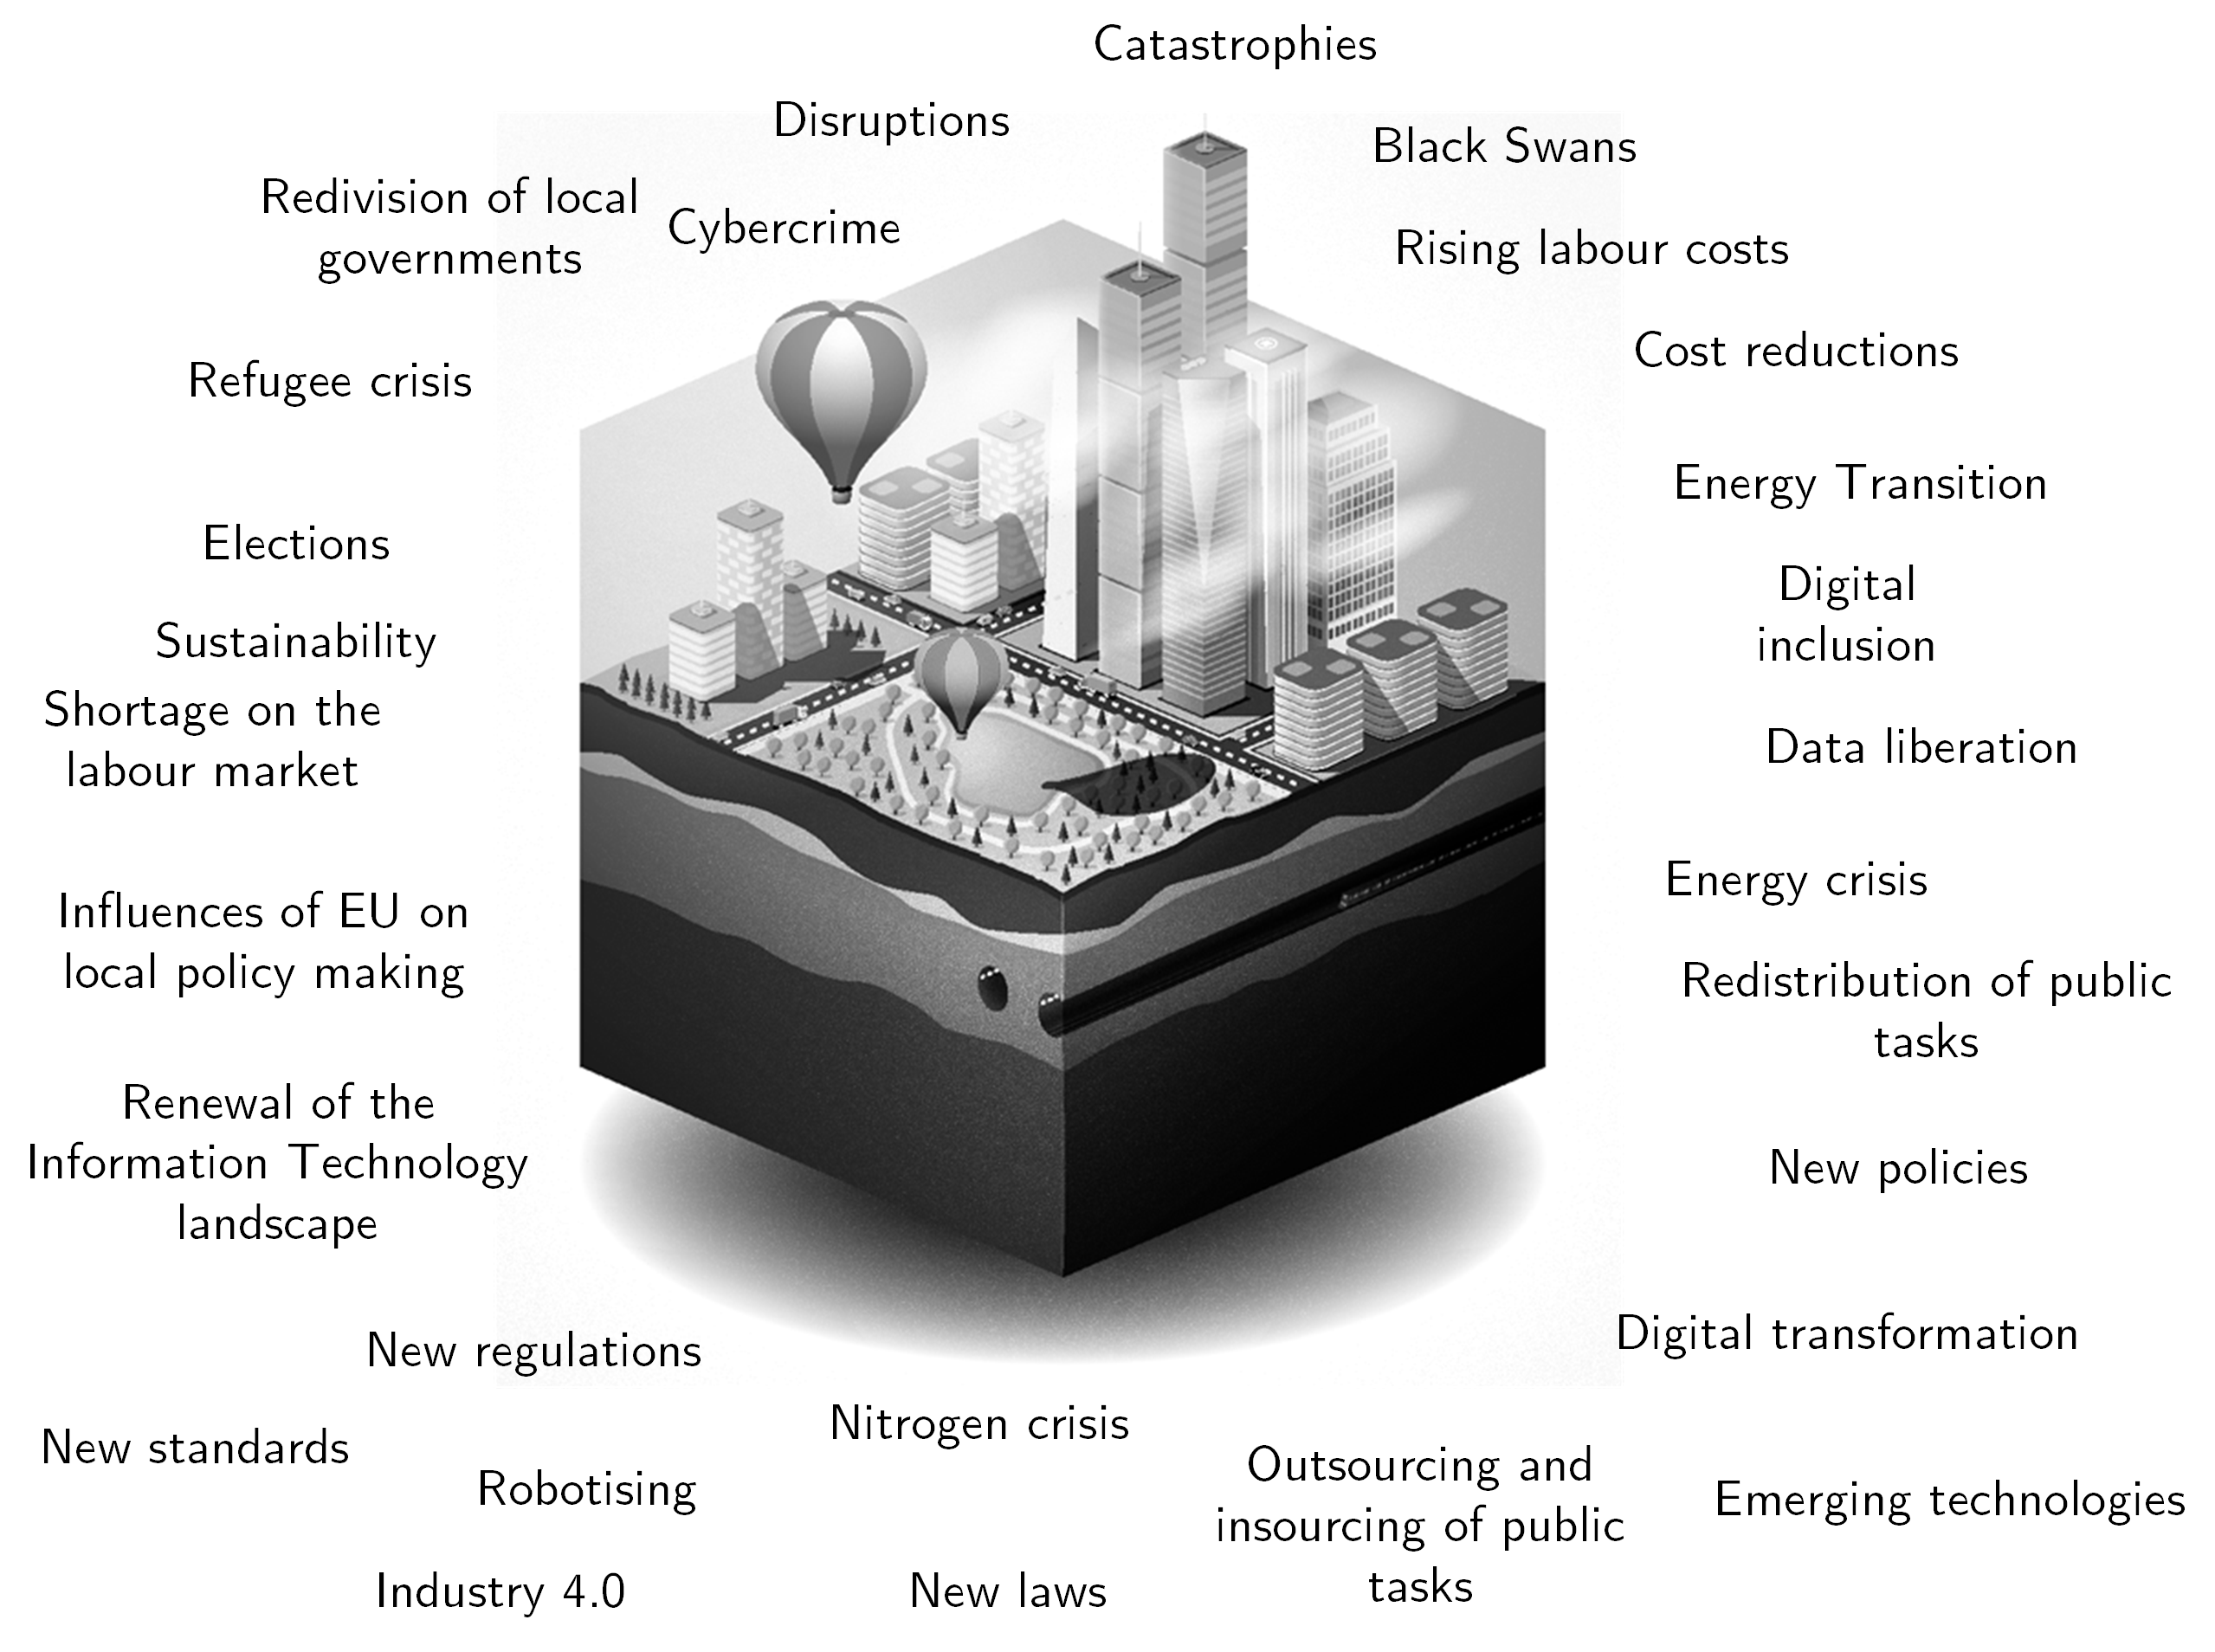
\includegraphics[width=0.8\linewidth]{images/publicstressors}
	\caption[Examples of stressors on the public sector]{Examples of stressors on the public sector}
	\label{fig:publicstressors}
\end{figure}
Because of the \gls{digitaltransformation}, the pace of change is increasing rapidly. In a study by \textcite{Eggers2015}, 96\% of respondents said digital technologies are significantly disrupting the \gls{ps}. According to \textcite{Nurmi2021}, organisations in the public and private sectors alike face the need to manage themselves in an ever more interconnected and fast-paced world. \textcite{Guggenberger2020} states that a paradigmatic change from a mechanistic toward a systemic worldview is ongoing, emphasizing the interconnectedness of participating organizations. 

\begin{remark}
	''The processes, while solid, cannot withstand the current pace of change; the dependence on emergency solutions and manual work is increasing'' \parencite[p.~2]{Wiebes2014}.
\end{remark}

The \gls{digitaltransformation} is not the only \gls{stressor} on the \gls{ps}. There are a lot of internal and external \glspl{stressor}. By being more \gls{robust} or \gls{resilient}, you can only withstand the change or the \gls{stressor}, but you do not gain from it. Governmental organisations and agencies in the Dutch \gls{ps} are searching for methods of dealing with this increased pace and the stressors. There are a lot of indications of this in the discussions and sessions held at \textcite{iBestuurterugblik2021}. The relevance of this research is not only about adding to the \acrshort{bok} of \acrshort{ea} and \gls{complexityscience} but also, in the context of public responsibility, to share the outcome with the \gls{ps} for further study and use.

\section{Design of the thesis}
\label{sec:structure}
The structure of this thesis follows a pattern of divergence before convergence (\cref{fig:design}). We introduce the research (\cref{ch:introduction}). We present the context, explain the design of the thesis, and the necessity of the research. Following, we introduce the main concepts of the research together with a problem statement and research questions. We give a background on the concepts of the research (\cref{ch:theoreticalbackground}). This part also contains the outcome of the literature research we performed based on the approach described in the methodology (\cref{ch:methodology}). The methodology explains the research design, the methods, the quality and the approach. All of these are part of the divergence of the research. We collected much data, but we still have to validate the data and narrow it down to formulate an answer to our research question. The second part of the thesis design will converge the findings.
\begin{figure}[H]
	\centering
	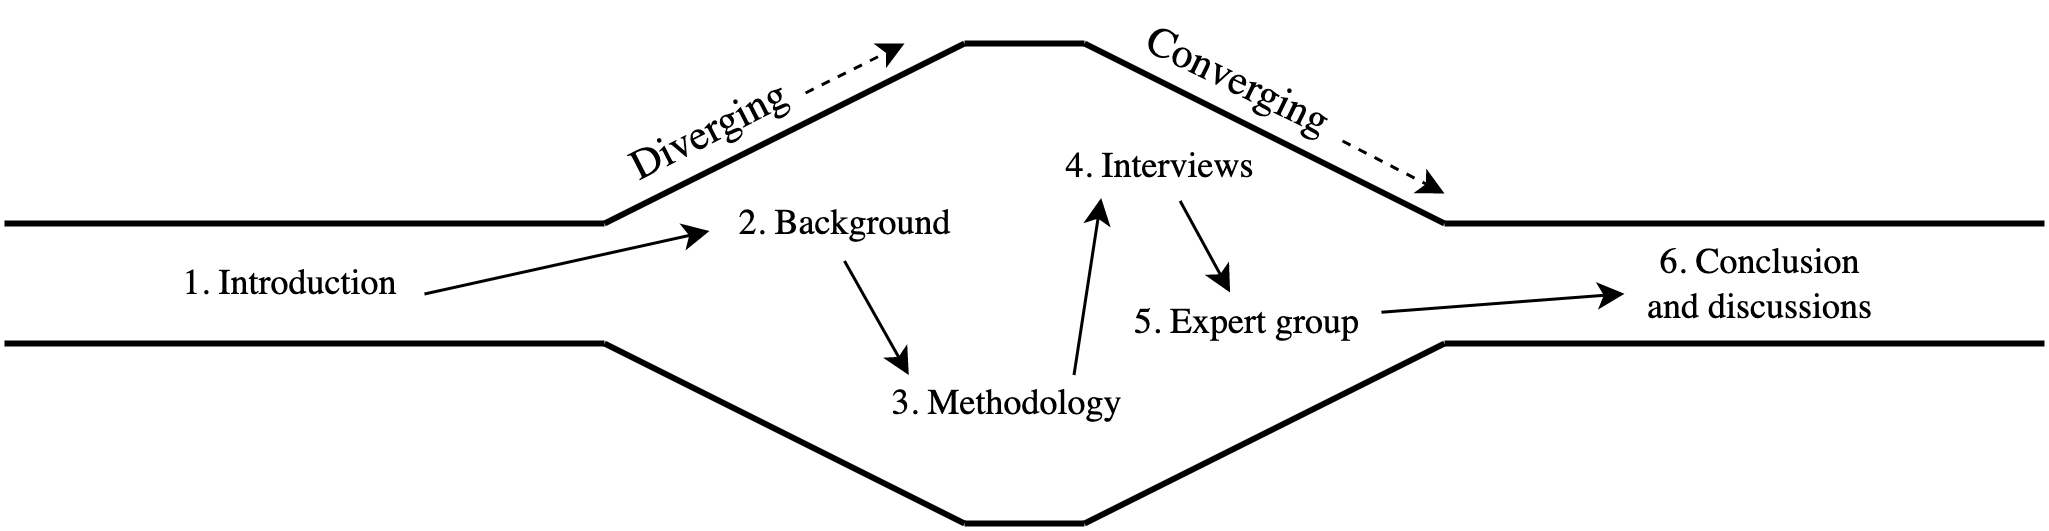
\includegraphics[width=0.9\linewidth]{images/structure}
	\caption[Design of the thesis]{Structure of the thesis}
	\label{fig:design}
\end{figure}
We validate findings with interviews (\cref{ch:interviews}) and an expert group (\cref{ch:expertgroup}). Converging ends with  conclusion and discussions (\cref{ch:conclusionanddiscussions}). The final part of the thesis design is a retrospective of the researcher, the research, and its process (\cref{ch:retrospective}). We have a glossary of terms available at the tail of the thesis to support the reader with used definitions.
